% arara: xelatex: { synctex: yes }
\documentclass[tikz]{standalone}
\usepackage{fontspec}
\usepackage{zxjatype}
\setCJKmainfont{ヒラギノ角ゴシック W3}

\usepackage{tikz}
\usetikzlibrary{
  circuits.logic.US, 
  positioning, 
  calc, 
  arrows.meta
  }
% ---- Common style (optional) ----
\tikzset{
  >=Latex,
  wire/.style={line width=0.8pt},
  lab/.style={font=\small},
  gatetitle/.style={font=\small\bfseries},
}
\usepackage[dvipsnames]{xcolor}




\begin{document}
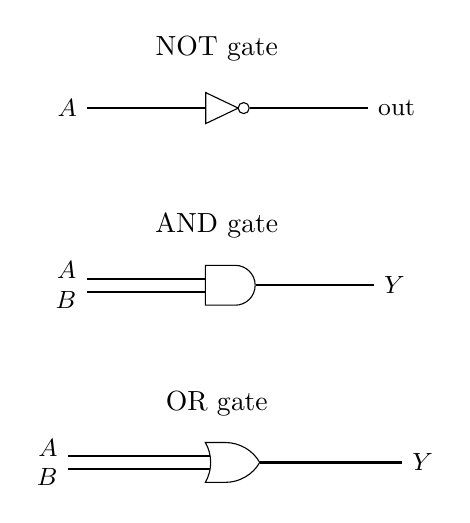
\begin{tikzpicture}[scale = 1.5]
% =========================================================
% (A) NOT gate
% =========================================================
  \node at (0,0.5) {NOT gate}; 
  \node[not gate US, draw, logic gate inputs=n] (not1) {};
  \draw[wire] (not1.input) -- ++(-1,0) node[left,lab] {$A$};
  \draw[wire] (not1.output) -- ++(1,0) node[right,lab] {out};
  % \node[gatetitle, above=2mm of not1] {NOT};
% =========================================================
% (B) AND gate (2-input)
% =========================================================
  \node at (0,-1) {AND gate}; 
  \node[and gate US, draw, logic gate inputs=nn] (and1) at (0.1,-1.5) {};
  \draw[wire] (and1.input 1) -- ++(-1,0) node[left,lab,yshift=3pt] {$A$};
  \draw[wire] (and1.input 2) -- ++(-1,0) node[left,lab,yshift=-3pt] {$B$};
  \draw[wire] (and1.output) -- ++(1,0) node[right,lab] {$Y$};
% =========================================================
% (C) OR gate (2-input)
% =========================================================
  \node at (0,-2.5) {OR gate}; 
  \node[or gate US, draw, logic gate inputs=nn] (or1) at (0.1,-3) {};
  \draw[wire] (or1.input 1) -- ++(-1.2,0) node[left,lab,yshift=3pt] {$A$};
  \draw[wire] (or1.input 2) -- ++(-1.2,0) node[left,lab,yshift=-3pt] {$B$};
  \draw[wire] (or1.output) -- ++(1.2,0) node[right,lab] {$Y$};
\end{tikzpicture} 

\end{document}